\documentclass{standalone}
\usepackage{tikz}
\usepackage{ctex,siunitx}
\setCJKmainfont{Noto Serif CJK SC}
\usepackage{tkz-euclide}
\usepackage{amsmath}
\usetikzlibrary{patterns, calc,3d}
\usetikzlibrary {decorations.pathmorphing,decorations.pathreplacing,decorations.shapes}
\begin{document}
\small
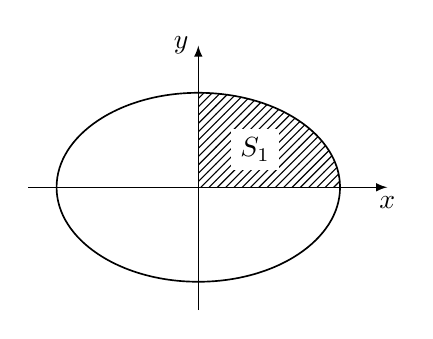
\begin{tikzpicture}[>=latex,scale=1.2]
  \draw[->](-1.8,0)--(2.0,0)node[below]{$x$};
  \draw[->](0,-1.3)--(0,1.5)node[left]{$y$};
  \draw[semithick](0,0)ellipse(1.5 and 1.0);
  \fill[pattern=north east lines](0,0)--(1.5,0)arc(0:90:1.5 and 1.0);
  \node at (0.6,0.4)[fill=white]{$S_1$};
\end{tikzpicture}
\end{document}